% Preambulo compartido para clases en formato beamer
\documentclass[9pt, xcolor=svgnames]{beamer}
\usepackage[utf8]{inputenc}
\usepackage[T1]{fontenc}
\usepackage[spanish,es-nodecimaldot]{babel}

\usetheme[progressbar=frametitle]{metropolis}
\metroset{sectionpage=none, subsectionpage=none}
\usepackage{appendixnumberbeamer}
\usepackage{booktabs}
\usepackage{amsmath,amssymb,bm,mathtools}
\usepackage{physics}
\usepackage{graphicx}
\usepackage{multicol}
\usepackage{tikz}
\usepackage{minted}
\usemintedstyle{tango}
\setminted{fontsize=\scriptsize, breaklines=true, linenos=true, bgcolor=LightGray!20, frame=lines}
\newminted{python}{fontsize=\scriptsize, breaklines=true, linenos=true, bgcolor=LightGray!20, frame=lines}
\usepackage{pgfplots}
\pgfplotsset{compat=1.18}
\usepackage{ragged2e}
\usepackage{xspace}
\newcommand{\themename}{\textbf{\textsc{metropolis}}\xspace}

\setbeamercolor{block title}{bg=MidnightBlue!85, fg=white}
\setbeamercolor{block body}{bg=MidnightBlue!5, fg=black}
\setbeamercolor{alerted text}{fg=Crimson}
\setbeamercolor{frametitle}{bg=MidnightBlue!10, fg=black}
\setbeamertemplate{blocks}[rounded][shadow=true]


\weektitle{07}{Autómatas celulares y Juego de la Vida de Conway}

\begin{document}

\frame{\titlepage}

\begin{frame}{Organización de la semana}
\begin{block}{Formato unificado}
La Semana 07 se divide en \textbf{Clase 1} y \textbf{Clase 2}, manteniendo la estructura habitual del curso:
\begin{itemize}
    \item \textbf{30--45 min} de teoría y discusión conceptual.
    \item \textbf{75--90 min} de laboratorio guiado con Python.
\end{itemize}
\end{block}

\vspace{0.2cm}
\begin{columns}[T,onlytextwidth]
\column{0.48\textwidth}
\textbf{Clase 1}
\begin{itemize}
    \item qué es un autómata celular;
    \item reglas locales, estados y vecindades;
    \item autómatas unidimensionales elementales;
    \item patrones, propagación de información y complejidad.
\end{itemize}

\column{0.48\textwidth}
\textbf{Clase 2}
\begin{itemize}
    \item autómatas bidimensionales;
    \item reglas de nacimiento y supervivencia;
    \item implementación del Juego de la Vida;
    \item análisis de patrones y fenómenos emergentes.
\end{itemize}
\end{columns}
\end{frame}

\section{Clase 1}

\begin{frame}[plain]
\centering
\vfill
{\Huge \bfseries Clase 1}\\[0.4cm]
{\Large Reglas locales, autómatas elementales y complejidad emergente}
\vfill
\end{frame}

\begin{frame}{Objetivos de la Clase 1}
\begin{itemize}
    \item Entender un autómata celular como un modelo discreto de espacio, tiempo y estado.
    \item Identificar la diferencia entre \textbf{regla local} y \textbf{comportamiento global}.
    \item Implementar autómatas celulares elementales en una dimensión.
    \item Comparar reglas que producen orden, periodicidad y comportamiento complejo.
\end{itemize}
\end{frame}

\begin{frame}{¿Qué es un autómata celular?}
\justifying
Un autómata celular (AC) es un sistema dinámico discreto definido por:
\begin{enumerate}
    \item una grilla de celdas;
    \item un conjunto finito de estados por celda;
    \item una vecindad local;
    \item una regla de actualización aplicada en pasos de tiempo.
\end{enumerate}

\begin{equation*}
\text{estado nuevo de una celda} = F(\text{estado local actual}).
\end{equation*}

\begin{alertblock}{Idea clave}
La evolución completa del sistema emerge de repetir muchas veces una regla simple aplicada en todas las celdas al mismo tiempo.
\end{alertblock}
\end{frame}

\begin{frame}{Por qué son interesantes en física y computación}
\begin{columns}[T]
\begin{column}{0.54\textwidth}
\begin{itemize}
    \item Sirven para estudiar \textbf{emergencia}: patrones macroscópicos desde interacciones microscópicas.
    \item Son modelos baratos computacionalmente y fáciles de paralelizar.
    \item Permiten explorar difusión, propagación, crecimiento, tráfico, incendios o ecología espacial.
    \item Son un puente natural entre física estadística, algoritmos y simulación.
\end{itemize}
\end{column}
\begin{column}{0.46\textwidth}
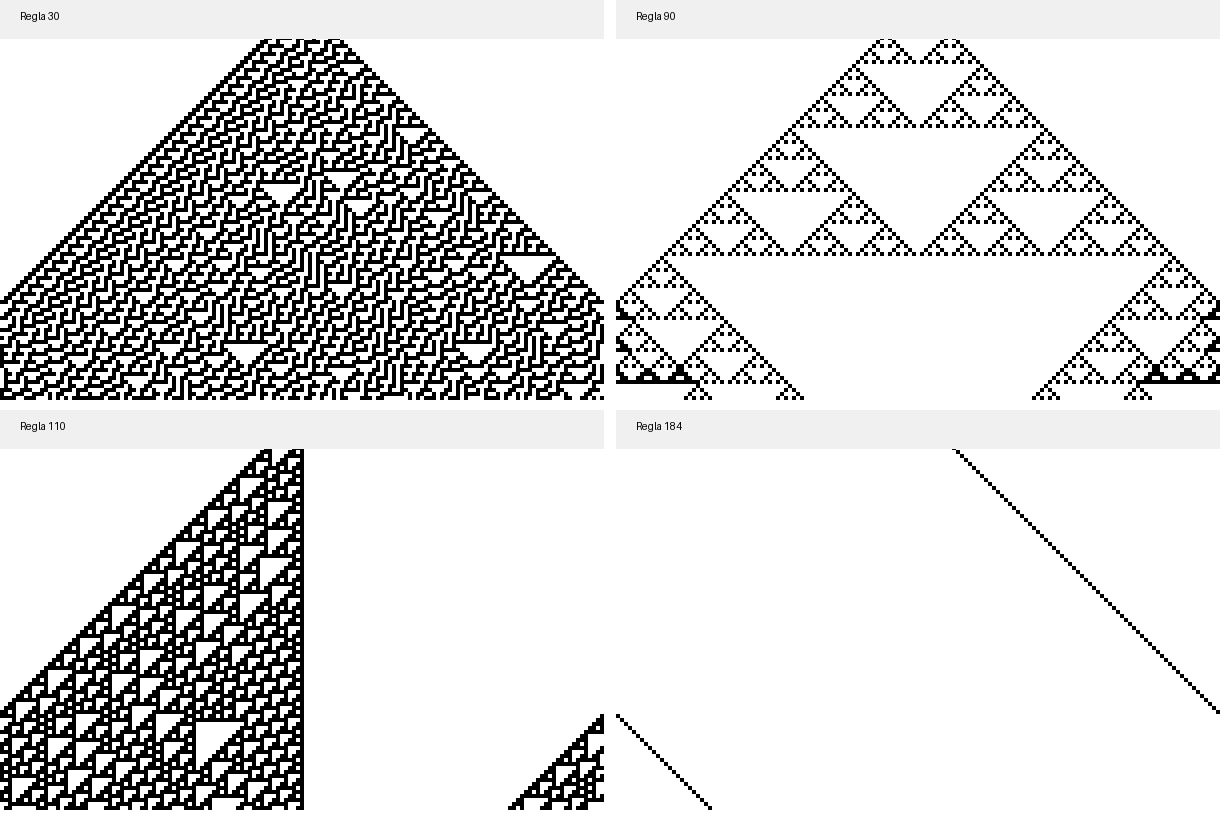
\includegraphics[width=\linewidth]{eca_gallery.png}
\end{column}
\end{columns}
\end{frame}

\begin{frame}{Ingredientes mínimos de un autómata elemental}
\begin{columns}[T]
\begin{column}{0.58\textwidth}
\begin{itemize}
    \item Grilla unidimensional de sitios $i=1,\dots,N$.
    \item Estados binarios: $s_i(t)\in\{0,1\}$.
    \item Vecindad de radio 1: izquierda, centro, derecha.
    \item Actualización sincrónica:
    \[
    s_i(t+1)=F\big(s_{i-1}(t),s_i(t),s_{i+1}(t)\big).
    \]
\end{itemize}
\end{column}
\begin{column}{0.42\textwidth}
\centering
\begin{tikzpicture}[scale=0.9]
    \foreach \x/\txt in {0/$s_{i-1}$,1.2/$s_i$,2.4/$s_{i+1}$} {
        \draw[fill=MidnightBlue!12] (\x,0) rectangle ++(1,1);
        \node at (\x+0.5,0.5) {\txt};
    }
    \node at (1.7,-0.7) {$\Downarrow$};
    \draw[fill=Crimson!15] (1.2,-2.2) rectangle ++(1,1);
    \node at (1.7,-1.7) {$s_i(t+1)$};
\end{tikzpicture}
\end{column}
\end{columns}
\end{frame}

\begin{frame}{Reglas elementales de Wolfram}
\small
Como la vecindad tiene tres celdas binarias, existen
\[
2^3 = 8
\]
configuraciones locales posibles.

Para cada configuración, la regla decide si el nuevo estado será $0$ o $1$.
Por eso el número total de reglas es
\[
2^8 = 256.
\]

\begin{block}{Codificación}
Una regla se identifica con un número entre $0$ y $255$. Por ejemplo, la regla 30 y la regla 110 son famosas por producir patrones ricos y difíciles de anticipar visualmente.
\end{block}
\end{frame}

\begin{frame}{Orden, periodicidad y complejidad}
\begin{itemize}
    \item Algunas reglas eliminan rápidamente toda actividad y llevan al sistema a un estado homogéneo.
    \item Otras producen patrones periódicos o altamente simétricos.
    \item Algunas generan estructuras móviles, choques y regiones aparentemente aleatorias.
\end{itemize}

\begin{block}{Pregunta central}
¿Qué rasgos de una regla local favorecen transmisión de información, memoria o interacción entre estructuras?
\end{block}

\begin{alertblock}{Lectura computacional}
Los autómatas celulares son laboratorios ideales para explorar cómo una implementación muy simple puede producir dinámica global no trivial.
\end{alertblock}
\end{frame}

\begin{frame}{Ejemplo: regla 30}
\begin{columns}[T]
\begin{column}{0.48\textwidth}
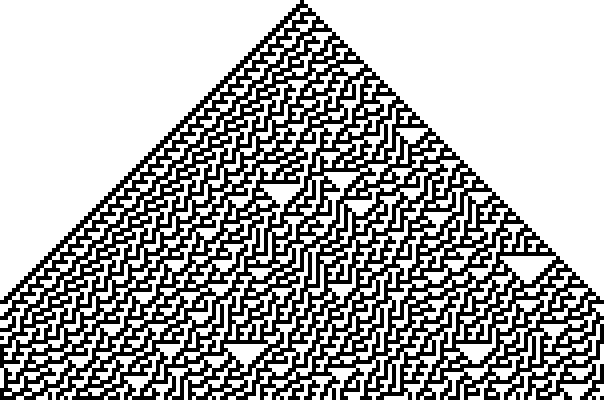
\includegraphics[width=\linewidth]{eca_rule30.png}
\end{column}
\begin{column}{0.52\textwidth}
\begin{itemize}
    \item Parte desde una sola celda activa.
    \item Genera una mezcla de simetría y aparente aleatoriedad.
    \item Se ha usado como ejemplo de generación pseudoaleatoria.
\end{itemize}

\begin{block}{Observación}
Aunque la regla es totalmente determinista, la textura espacial puede parecer caótica.
\end{block}
\end{column}
\end{columns}
\end{frame}

\begin{frame}[fragile]{Código base: autómata elemental 1D}
\inputminted[firstline=1,lastline=27]{python}{codes/elementary_ca.py}
\end{frame}

\begin{frame}[fragile]{Código de apoyo: comparar varias reglas}
\inputminted[firstline=1,lastline=21]{python}{codes/rule_gallery.py}
\end{frame}

\begin{frame}[fragile]{Código de apoyo: renderizar el patrón}
\inputminted[firstline=30,lastline=42]{python}{codes/elementary_ca.py}
\end{frame}

\begin{frame}{Actividades propuestas para la Clase 1}
\begin{enumerate}
    \item Simular las reglas 30, 90, 110 y 184 desde una condición inicial puntual.
    \item Repetir el experimento con condición inicial aleatoria.
    \item Describir visualmente qué reglas parecen más ordenadas y cuáles más complejas.
    \item Proponer una métrica simple: fracción de celdas activas, ancho del patrón o número de transiciones $0\leftrightarrow1$.
\end{enumerate}

\begin{block}{Entregable sugerido}
Script o notebook con figuras, comparación entre reglas y una breve interpretación sobre propagación, simetría y complejidad.
\end{block}
\end{frame}

\begin{frame}{Cierre Clase 1}
\begin{itemize}
    \item Un autómata celular traduce una regla local discreta en una evolución espacio-temporal completa.
    \item Las reglas elementales muestran que incluso en 1D aparece una gran diversidad de comportamientos.
    \item La siguiente pregunta natural es qué ocurre al pasar a dos dimensiones.
\end{itemize}
\end{frame}

\section{Clase 2}

\begin{frame}[plain]
\centering
\vfill
{\Huge \bfseries Clase 2}\\[0.4cm]
{\Large Juego de la Vida: patrones bidimensionales y emergencia}
\vfill
\end{frame}

\begin{frame}{Objetivos de la Clase 2}
\begin{itemize}
    \item Entender la regla del Juego de la Vida como un autómata bidimensional.
    \item Implementar conteo de vecinos y actualización sincrónica en una grilla 2D.
    \item Reconocer patrones típicos: still lifes, osciladores y naves.
    \item Analizar cómo reglas muy cortas producen estructuras persistentes y móviles.
\end{itemize}
\end{frame}

\begin{frame}{Del caso 1D al caso 2D}
\justifying
En el caso bidimensional, cada celda ocupa una posición $(i,j)$ en una grilla y su
vecindad más común es la de Moore: las ocho celdas que la rodean.

\begin{equation*}
s_{ij}(t+1)=F\big(\text{vecinos de } (i,j)\big).
\end{equation*}

\begin{itemize}
    \item La estructura espacial es más rica que en 1D.
    \item Aparecen objetos localizados que interactúan entre sí.
    \item La visualización se vuelve una herramienta central para entender la dinámica.
\end{itemize}
\end{frame}

\begin{frame}{Reglas del Juego de la Vida de Conway}
\begin{block}{Estados}
Cada celda está \textbf{viva} ($1$) o \textbf{muerta} ($0$).
\end{block}

\begin{block}{Actualización}
Sea $n$ el número de vecinos vivos:
\begin{itemize}
    \item una celda viva sobrevive si $n=2$ o $n=3$;
    \item una celda muerta nace si $n=3$;
    \item en cualquier otro caso, la celda queda o pasa a muerta.
\end{itemize}
\end{block}

\begin{alertblock}{Notación compacta}
Se suele resumir como \texttt{B3/S23}: birth con 3 vecinos, survival con 2 o 3.
\end{alertblock}
\end{frame}

\begin{frame}{Qué tipos de patrones aparecen}
\begin{columns}[T]
\begin{column}{0.52\textwidth}
\begin{itemize}
    \item \textbf{Still lifes}: configuraciones estáticas como el bloque.
    \item \textbf{Osciladores}: repiten una forma tras algunos pasos, como el blinker.
    \item \textbf{Naves}: se desplazan por la grilla, como el glider.
    \item \textbf{Semillas activas}: estructuras que evolucionan por mucho tiempo antes de estabilizarse.
\end{itemize}
\end{column}
\begin{column}{0.48\textwidth}
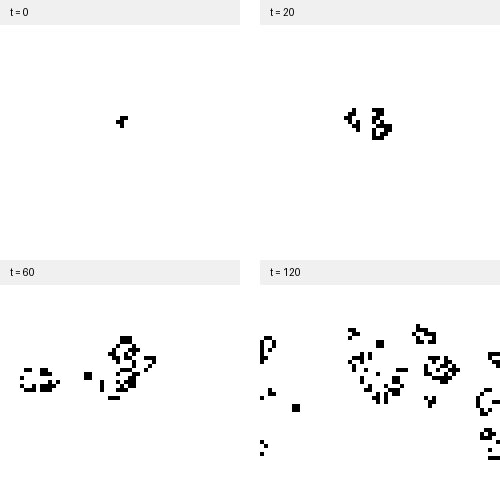
\includegraphics[width=\linewidth]{life_evolution.png}
\end{column}
\end{columns}
\end{frame}

\begin{frame}{Lectura física del modelo}
\begin{itemize}
    \item No es un modelo realista de biología en detalle.
    \item Sí captura una idea muy valiosa: \textbf{interacción local + umbrales} puede generar patrones globales robustos.
    \item Permite discutir estabilidad, propagación, colisiones y sensibilidad al estado inicial.
\end{itemize}

\begin{block}{Conexión con el curso}
El Juego de la Vida es un ejemplo excelente de modelación computacional: definimos un sistema discreto, lo implementamos, lo visualizamos y luego interpretamos su dinámica.
\end{block}
\end{frame}

\begin{frame}{Flujo de implementación}
\small
\begin{enumerate}
    \item Definir una matriz binaria para el estado inicial.
    \item Contar vecinos vivos para cada celda.
    \item Construir una nueva matriz aplicando las reglas de Conway.
    \item Repetir por muchos pasos y guardar instantáneas.
    \item Analizar si el sistema muere, se estabiliza, oscila o sigue produciendo actividad.
\end{enumerate}

\begin{alertblock}{Decisión de modelamiento}
Una condición periódica de borde convierte la grilla en un toro y evita que las estructuras ``desaparezcan'' por los bordes.
\end{alertblock}
\end{frame}

\begin{frame}[fragile]{Código base: conteo de vecinos y actualización}
\inputminted[firstline=1,lastline=20]{python}{codes/game_of_life.py}
\end{frame}

\begin{frame}[fragile]{Código de apoyo: semillas iniciales}
\inputminted[firstline=23,lastline=43]{python}{codes/game_of_life.py}
\end{frame}

\begin{frame}[fragile]{Código de apoyo: simulación e instantáneas}
\inputminted[firstline=46,lastline=62]{python}{codes/game_of_life.py}
\end{frame}

\begin{frame}{Actividades propuestas para la Clase 2}
\begin{enumerate}
    \item Implementar el Juego de la Vida con bordes periódicos.
    \item Probar al menos tres semillas: glider, blinker y R-pentomino.
    \item Medir el número de celdas vivas en función del tiempo.
    \item Identificar si el patrón converge a reposo, oscilación o propagación.
    \item Desafío: comparar con una variante de reglas, por ejemplo \texttt{B36/S23}.
\end{enumerate}

\begin{block}{Entregable sugerido}
Notebook o script con imágenes de la evolución, un gráfico de población viva y una discusión breve sobre patrones emergentes.
\end{block}
\end{frame}

\begin{frame}{Preguntas guía para cerrar la semana}
\begin{itemize}
    \item ¿Qué cambia al pasar de reglas 1D a una dinámica 2D?
    \item ¿Por qué algunas estructuras sobreviven y otras colapsan rápidamente?
    \item ¿Qué significa aquí ``complejidad'' y cómo podríamos medirla?
    \item ¿Qué otras aplicaciones podrían modelarse con reglas locales en una grilla?
\end{itemize}
\end{frame}

\begin{frame}{Cierre de la semana}
\begin{itemize}
    \item Los autómatas celulares muestran cómo reglas locales discretas generan patrones espacio-temporales ricos.
    \item Las reglas elementales son una puerta de entrada simple a la idea de emergencia.
    \item El Juego de la Vida cierra la semana conectando implementación, visualización y análisis de comportamiento colectivo.
\end{itemize}

\vspace{0.2cm}
\centering
\textbf{Próximo paso natural:} medir observables y comparar familias de reglas más allá de Conway.
\end{frame}

\end{document}
